\documentclass{article}
\title{\LaTeX Math notes}
\author{Samuel Hautamäki}
\date{th of October 2024}
\usepackage{mathtools,amssymb,amsthm,gensymb,textcomp}
\usepackage{graphicx}
\graphicspath{ {./} }

\begin{document}
  \maketitle
   
  \section{sin cos or tan functions}
  HL P 410, SL p523\\
  $f(x)=\sin x$\\
  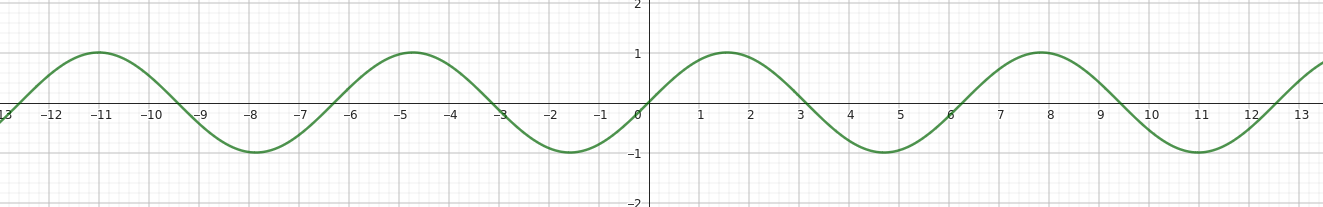
\includegraphics {sinewave}
  where x in radian unit!\\
  domain: $\in\mathbb{R}$\\
  range $-1\leq y\leq 1 or [-1,1]$\\
  sin x is periodic function. $\sin(x)=\sin(x+2\pi\cdot n)$\\
  repeats the same y-values after $2\pi$.\\
  amplitude=$\frac{max-min}{2}=1$\\
  and sine function passes point (0,0) so $\sin(0)=0$\\
  2) $g(x)=\cos(x)$ where x is real number in radian - unit.\\
  just like $\sin x$ but a bit to the left.\\
  $\sin(0)=1$\\
  domain: $x\in\mathbb{R}$\\
  $range: -1\leq y\leq 1$\\
  periodic $\cos(x)=\cos(x+2\pi\cdot n)$ and passes point (0,1)\\
  3) and $y=\sin(x)+d$\\
  $d>0 moves up$\\
  $d<0 moves down$\\
  4) $a\cdot \sin(x)$\\
  a changes amplitude min/max\\
  $a<0$ reflects about x-axis\\
  5) $\sin(b\cdot x) or \cos(b\cdot x)$\\
  b changes period $b=\frac{2\pi}{period}$.\\
  $b<0$ reflects about y-axis\\
  6) $\sin(x+c) or \cos(x+c)$\\
  $c>0$ moves to right\\
  $c<0$ moves to left\\
  7) tangent function $h(x)=\tan(x)$\\
  x is real number, radian unit!\\
  domain:$x\neq\frac{\pi}{2}+n\cdot\pi$\\
  range:y is $\in\mathbb{R}$\\
  period:\pi for tangent so $\tan(x)=\tan(x+\pi\cdot n)$\\
  excercoses sl12g+12i\\
  hl ex6n p414\\
  \subsection{ex 6n}
  1. $cosec=\frac{1}{\sin}$
  $f(\theta)=\sin\theta$\\
  $g(\theta)=\frac{1}{\sin\theta}$.\\
  It is inverse. And it has asymptotes\\
  2. $f(\theta)=\tan\theta$\\
  $f(\theta)=\frac{1}{\tan\theta}$\\
  It is inverse. (Swings the other way.)\\
  3.  



  

   
\end{document}
